% AUTO-GENERATED by code/figlib.py helpers -- do not edit
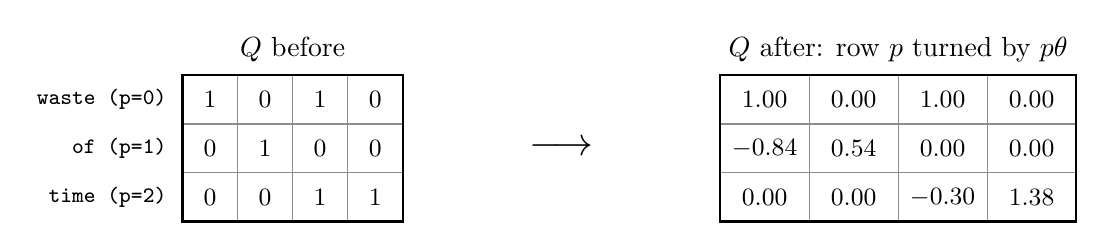
\begin{tikzpicture}
\draw[black!45, fill=white] (1.965,0.930) rectangle (2.665,0.310);
\node[font=\small, text=black] at (2.315,0.620) {$1$};
\draw[black!45, fill=white] (2.665,0.930) rectangle (3.365,0.310);
\node[font=\small, text=black] at (3.015,0.620) {$0$};
\draw[black!45, fill=white] (3.365,0.930) rectangle (4.065,0.310);
\node[font=\small, text=black] at (3.715,0.620) {$1$};
\draw[black!45, fill=white] (4.065,0.930) rectangle (4.765,0.310);
\node[font=\small, text=black] at (4.415,0.620) {$0$};
\draw[black!45, fill=white] (1.965,0.310) rectangle (2.665,-0.310);
\node[font=\small, text=black] at (2.315,-0.000) {$0$};
\draw[black!45, fill=white] (2.665,0.310) rectangle (3.365,-0.310);
\node[font=\small, text=black] at (3.015,-0.000) {$1$};
\draw[black!45, fill=white] (3.365,0.310) rectangle (4.065,-0.310);
\node[font=\small, text=black] at (3.715,-0.000) {$0$};
\draw[black!45, fill=white] (4.065,0.310) rectangle (4.765,-0.310);
\node[font=\small, text=black] at (4.415,-0.000) {$0$};
\draw[black!45, fill=white] (1.965,-0.310) rectangle (2.665,-0.930);
\node[font=\small, text=black] at (2.315,-0.620) {$0$};
\draw[black!45, fill=white] (2.665,-0.310) rectangle (3.365,-0.930);
\node[font=\small, text=black] at (3.015,-0.620) {$0$};
\draw[black!45, fill=white] (3.365,-0.310) rectangle (4.065,-0.930);
\node[font=\small, text=black] at (3.715,-0.620) {$1$};
\draw[black!45, fill=white] (4.065,-0.310) rectangle (4.765,-0.930);
\node[font=\small, text=black] at (4.415,-0.620) {$1$};
\draw[line width=0.9pt] (1.965,0.930) rectangle (4.765,-0.930);
\node[anchor=east, font=\footnotesize\ttfamily] at (1.885,0.620) {waste (p=0)};
\node[anchor=east, font=\footnotesize\ttfamily] at (1.885,-0.000) {of (p=1)};
\node[anchor=east, font=\footnotesize\ttfamily] at (1.885,-0.620) {time (p=2)};
\node[anchor=south, font=\normalsize] at (3.365,0.980) {$Q$ before};
\node[font=\Large] at (6.780,0) {$\longrightarrow$};
\draw[black!45, fill=white] (8.795,0.930) rectangle (9.925,0.310);
\node[font=\small, text=black] at (9.360,0.620) {$1.00$};
\draw[black!45, fill=white] (9.925,0.930) rectangle (11.055,0.310);
\node[font=\small, text=black] at (10.490,0.620) {$0.00$};
\draw[black!45, fill=white] (11.055,0.930) rectangle (12.185,0.310);
\node[font=\small, text=black] at (11.620,0.620) {$1.00$};
\draw[black!45, fill=white] (12.185,0.930) rectangle (13.315,0.310);
\node[font=\small, text=black] at (12.750,0.620) {$0.00$};
\draw[black!45, fill=white] (8.795,0.310) rectangle (9.925,-0.310);
\node[font=\small, text=black] at (9.360,-0.000) {$-0.84$};
\draw[black!45, fill=white] (9.925,0.310) rectangle (11.055,-0.310);
\node[font=\small, text=black] at (10.490,-0.000) {$0.54$};
\draw[black!45, fill=white] (11.055,0.310) rectangle (12.185,-0.310);
\node[font=\small, text=black] at (11.620,-0.000) {$0.00$};
\draw[black!45, fill=white] (12.185,0.310) rectangle (13.315,-0.310);
\node[font=\small, text=black] at (12.750,-0.000) {$0.00$};
\draw[black!45, fill=white] (8.795,-0.310) rectangle (9.925,-0.930);
\node[font=\small, text=black] at (9.360,-0.620) {$0.00$};
\draw[black!45, fill=white] (9.925,-0.310) rectangle (11.055,-0.930);
\node[font=\small, text=black] at (10.490,-0.620) {$0.00$};
\draw[black!45, fill=white] (11.055,-0.310) rectangle (12.185,-0.930);
\node[font=\small, text=black] at (11.620,-0.620) {$-0.30$};
\draw[black!45, fill=white] (12.185,-0.310) rectangle (13.315,-0.930);
\node[font=\small, text=black] at (12.750,-0.620) {$1.38$};
\draw[line width=0.9pt] (8.795,0.930) rectangle (13.315,-0.930);
\node[anchor=south, font=\normalsize] at (11.055,0.980) {$Q$ after: row $p$ turned by $p\theta$};
\end{tikzpicture}
\\[10pt]
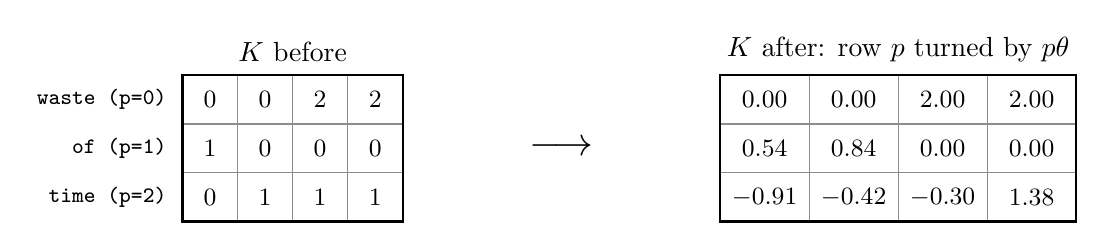
\begin{tikzpicture}
\draw[black!45, fill=white] (1.965,0.930) rectangle (2.665,0.310);
\node[font=\small, text=black] at (2.315,0.620) {$0$};
\draw[black!45, fill=white] (2.665,0.930) rectangle (3.365,0.310);
\node[font=\small, text=black] at (3.015,0.620) {$0$};
\draw[black!45, fill=white] (3.365,0.930) rectangle (4.065,0.310);
\node[font=\small, text=black] at (3.715,0.620) {$2$};
\draw[black!45, fill=white] (4.065,0.930) rectangle (4.765,0.310);
\node[font=\small, text=black] at (4.415,0.620) {$2$};
\draw[black!45, fill=white] (1.965,0.310) rectangle (2.665,-0.310);
\node[font=\small, text=black] at (2.315,-0.000) {$1$};
\draw[black!45, fill=white] (2.665,0.310) rectangle (3.365,-0.310);
\node[font=\small, text=black] at (3.015,-0.000) {$0$};
\draw[black!45, fill=white] (3.365,0.310) rectangle (4.065,-0.310);
\node[font=\small, text=black] at (3.715,-0.000) {$0$};
\draw[black!45, fill=white] (4.065,0.310) rectangle (4.765,-0.310);
\node[font=\small, text=black] at (4.415,-0.000) {$0$};
\draw[black!45, fill=white] (1.965,-0.310) rectangle (2.665,-0.930);
\node[font=\small, text=black] at (2.315,-0.620) {$0$};
\draw[black!45, fill=white] (2.665,-0.310) rectangle (3.365,-0.930);
\node[font=\small, text=black] at (3.015,-0.620) {$1$};
\draw[black!45, fill=white] (3.365,-0.310) rectangle (4.065,-0.930);
\node[font=\small, text=black] at (3.715,-0.620) {$1$};
\draw[black!45, fill=white] (4.065,-0.310) rectangle (4.765,-0.930);
\node[font=\small, text=black] at (4.415,-0.620) {$1$};
\draw[line width=0.9pt] (1.965,0.930) rectangle (4.765,-0.930);
\node[anchor=east, font=\footnotesize\ttfamily] at (1.885,0.620) {waste (p=0)};
\node[anchor=east, font=\footnotesize\ttfamily] at (1.885,-0.000) {of (p=1)};
\node[anchor=east, font=\footnotesize\ttfamily] at (1.885,-0.620) {time (p=2)};
\node[anchor=south, font=\normalsize] at (3.365,0.980) {$K$ before};
\node[font=\Large] at (6.780,0) {$\longrightarrow$};
\draw[black!45, fill=white] (8.795,0.930) rectangle (9.925,0.310);
\node[font=\small, text=black] at (9.360,0.620) {$0.00$};
\draw[black!45, fill=white] (9.925,0.930) rectangle (11.055,0.310);
\node[font=\small, text=black] at (10.490,0.620) {$0.00$};
\draw[black!45, fill=white] (11.055,0.930) rectangle (12.185,0.310);
\node[font=\small, text=black] at (11.620,0.620) {$2.00$};
\draw[black!45, fill=white] (12.185,0.930) rectangle (13.315,0.310);
\node[font=\small, text=black] at (12.750,0.620) {$2.00$};
\draw[black!45, fill=white] (8.795,0.310) rectangle (9.925,-0.310);
\node[font=\small, text=black] at (9.360,-0.000) {$0.54$};
\draw[black!45, fill=white] (9.925,0.310) rectangle (11.055,-0.310);
\node[font=\small, text=black] at (10.490,-0.000) {$0.84$};
\draw[black!45, fill=white] (11.055,0.310) rectangle (12.185,-0.310);
\node[font=\small, text=black] at (11.620,-0.000) {$0.00$};
\draw[black!45, fill=white] (12.185,0.310) rectangle (13.315,-0.310);
\node[font=\small, text=black] at (12.750,-0.000) {$0.00$};
\draw[black!45, fill=white] (8.795,-0.310) rectangle (9.925,-0.930);
\node[font=\small, text=black] at (9.360,-0.620) {$-0.91$};
\draw[black!45, fill=white] (9.925,-0.310) rectangle (11.055,-0.930);
\node[font=\small, text=black] at (10.490,-0.620) {$-0.42$};
\draw[black!45, fill=white] (11.055,-0.310) rectangle (12.185,-0.930);
\node[font=\small, text=black] at (11.620,-0.620) {$-0.30$};
\draw[black!45, fill=white] (12.185,-0.310) rectangle (13.315,-0.930);
\node[font=\small, text=black] at (12.750,-0.620) {$1.38$};
\draw[line width=0.9pt] (8.795,0.930) rectangle (13.315,-0.930);
\node[anchor=south, font=\normalsize] at (11.055,0.980) {$K$ after: row $p$ turned by $p\theta$};
\end{tikzpicture}
